\chapter{生体データを用いたコンテンツへの重畳提示システム}

\thispagestyle{myheadings}

 本章では生体データを使いコンテンツに重畳提示する手法について述べる.
図に研究の全体像を示す.システムの流れは,コンテンツを視聴しているときの生体データを取得する.
生体データはコンテンツ毎に収集する.集めた生体データから盛り上がっている箇所を推定し抜き出す.
抜き出したデータを基にコンテンツに重畳提示するといった構成である.

\begin{figure}[H]
    \centering
    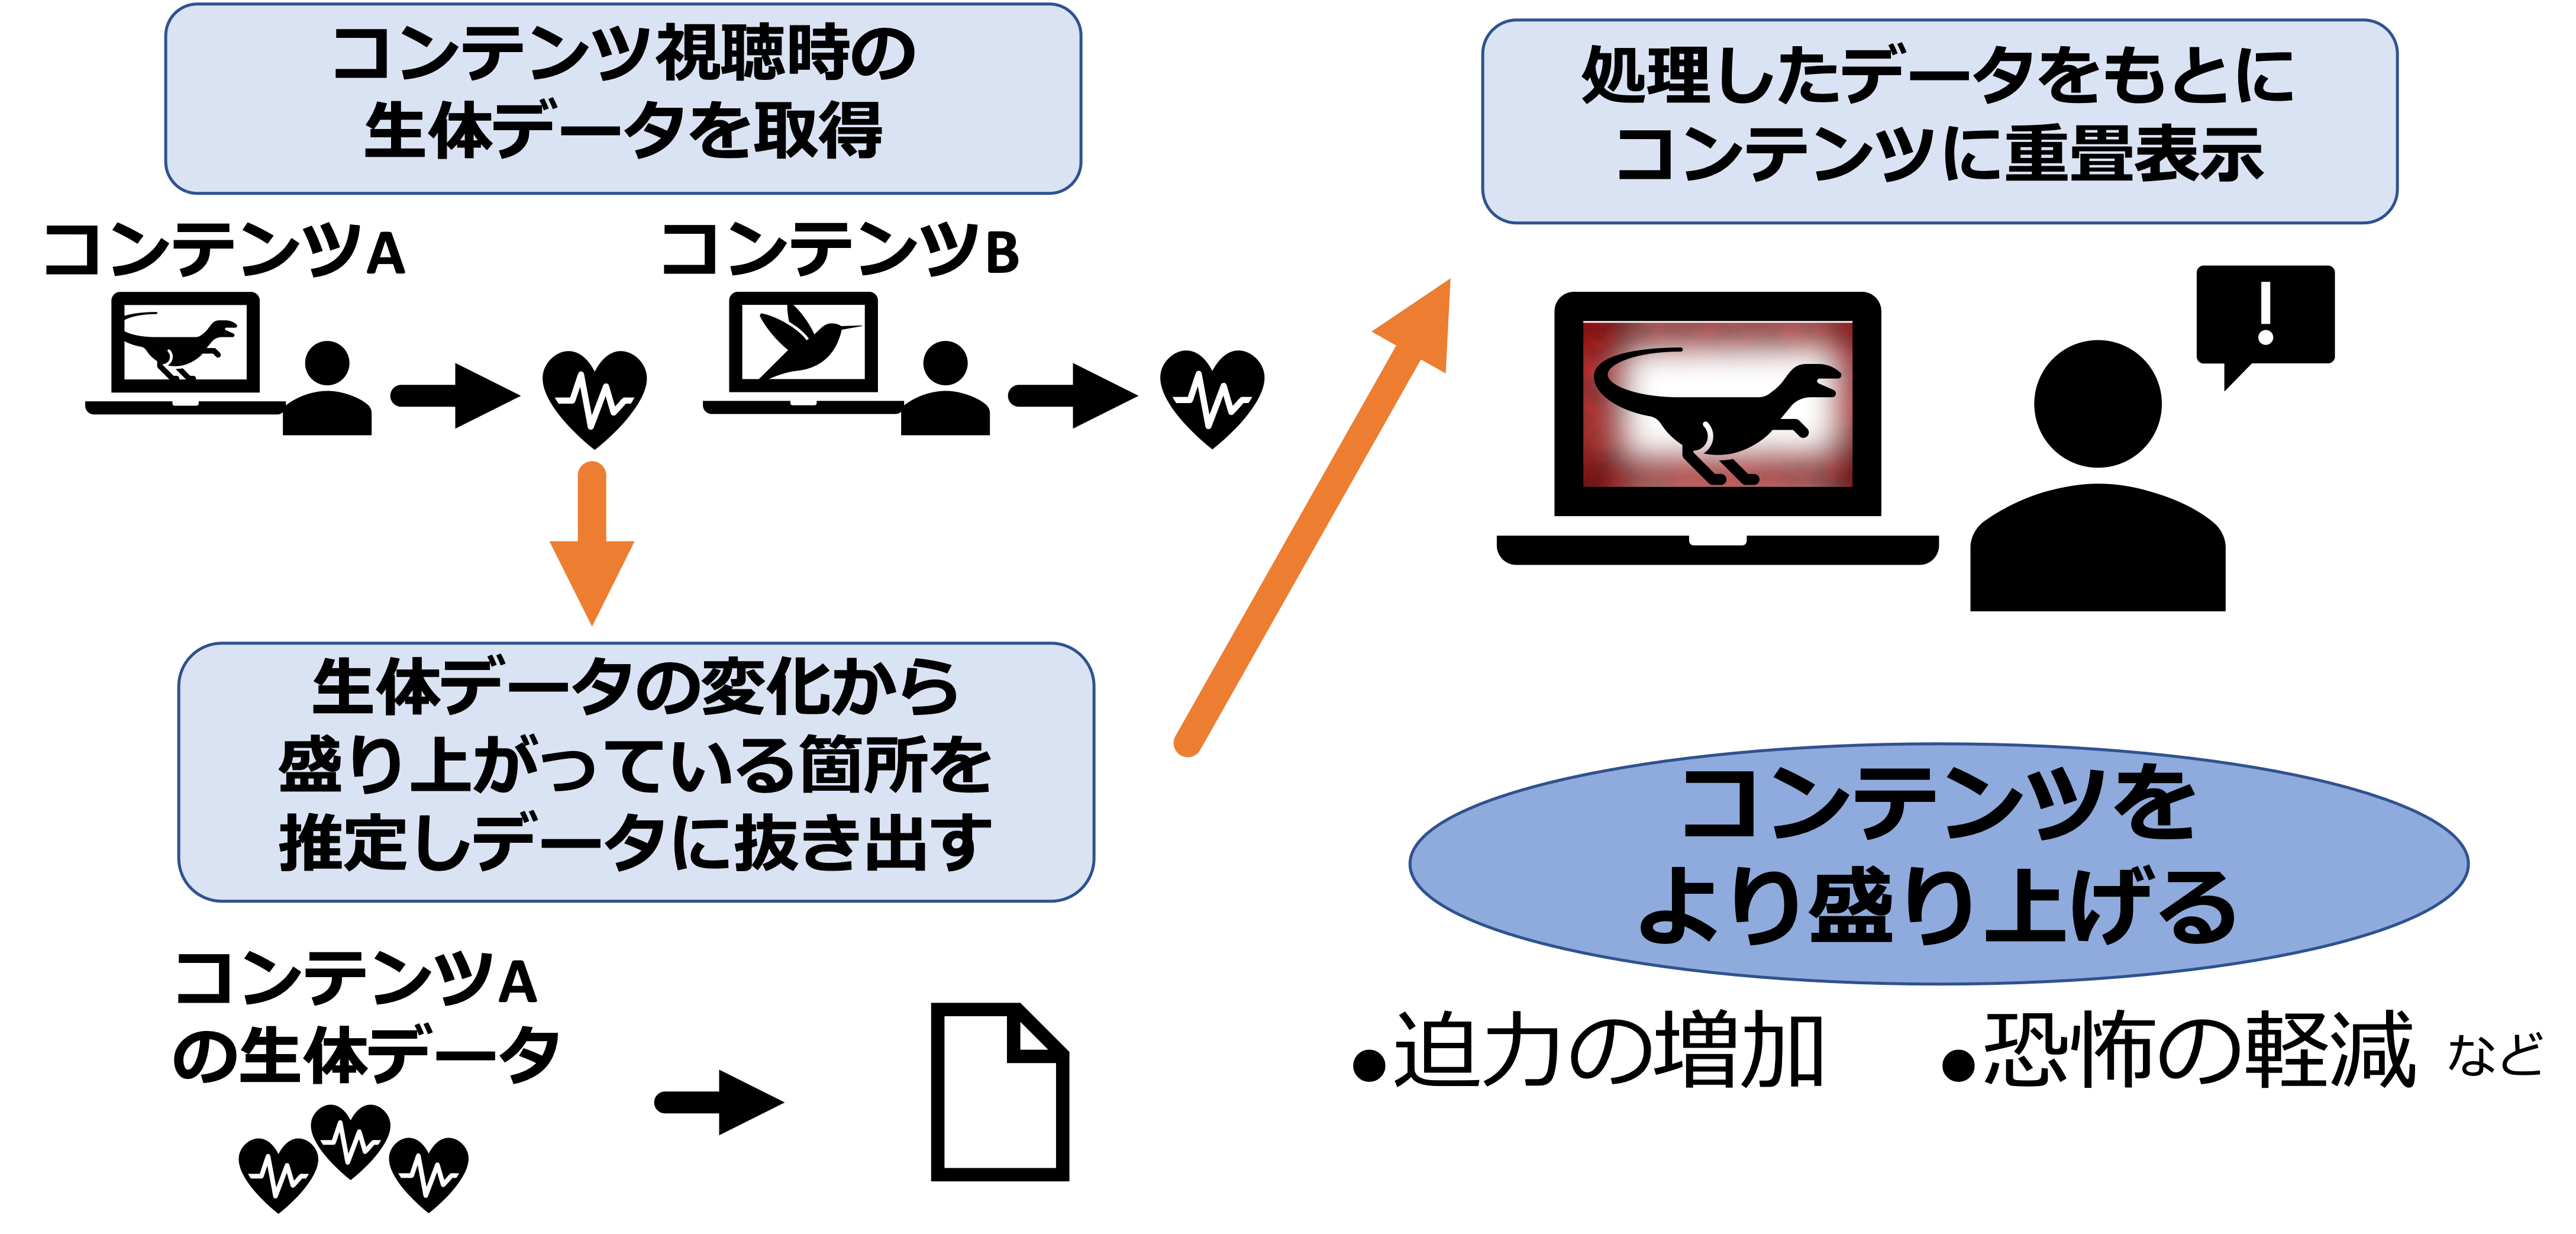
\includegraphics[width=15cm]{images/chapter3/allsysytem.png}
    \caption{システム全体図}
\end{figure}

 コンテンツ視聴時に生体データを取得する理由として,生体データを用いればそのコンテンツに対し視聴者が興奮している箇所を推定可能だからである.
本研究ではコンテンツの盛り上がっている箇所を複数人で共有するため,コンテンツのどの箇所で視聴者が盛り上がっていたのかを生体データを使って推定する.
コンテンツにエフェクトを重畳する目的として生体データを基にコンテンツにエフェクトを重畳することにより,
より盛り上がるコンテンツを楽しむことが可能になるからである.そのため本研究ではコンテンツ視聴時の生体データを取得し,
コンテンツにエフェクトを重畳するシステムにした.
 コンテンツを視聴している時の生体データについて述べる.
収集する生体データとして目の動きに注目したり,額から出る汗の量でコンテンツ視聴時の興奮度を測る方法などが考えられる.
収集する生体データによってコンテンツに対し盛り上がり方を色々な目線で計測するのが可能である.
さまざまな方法で生体データを収集するのができるため,視聴するコンテンツによって適した生体データを取得する.
コンテンツにはYouTubeやNetflixなどのデジタルコンテンツと本や新聞紙などのアナログコンテンツがある.
本研究のシステムではYouTubeなどを視聴している時の生体データの収集だけでなく,新聞紙や本を読んでいる時も盛り上がりポイントを計測するのが可能である.
例として新聞紙を読んでいる時,生体データとして額から出る汗や目の動きなどでは正確に盛り上がるポイントを見つけ出せない.
新聞紙を読んでいる時は心拍数を使い,面白いと感じる記事を読んでいるときの心拍数を計測するなどコンテンツに合わせた生体データを取得する.
またTwitterやInstagram,Facebook,TiktokなどのSNSコンテンツを視聴している時にも使用できる.
 コンテンツへの重畳手法について述べる.コンテンツへの重畳手法としては音を追加したり,画面にエフェクトを表示させる,
デバイスを振動させるなどさまざまである.映画館のような3Dや4DXは映画館の中の決められた映画のみだが,
本研究は生体データを収集すれば自宅でも好きなコンテンツに対し映像体験が可能になる.例として本を読んでいる時の重畳手法は,
徐々に部屋を暗くしたり雑音をはじめの方は流していて盛り上がるポイントが来たら無音にするなど集中しやすい環境に近づけていく.
その他にも音楽を聴いているときはサビにかけてボリュームを上げビートに合わせてデバイスを振動させライブ会場のようなワクワクが体験できたり,
スマートフォンで車のレースゲームをしている時には風を送りゲームに没入感を加える.

\section{本研究のシステム構成}
 本研究で採用したシステムについて述べる.本研究では生体データの収集方法としてスマートウォッチを採用した.
理由として近年スマートウォッチは普及しており,誰でも気軽に生体データを取得できるからである図.今回スマートウォッチはTicWatchE3を使用した[図].
コンテンツは映画を視聴することにした.コロナ禍により自宅で映画を視聴する機会が増えたためである.
また,映画は盛り上がるポイントが明確に出てくると予想したからである.スマートウォッチを使い映画を視聴している時の生体データとして,心拍数を計測する.
心拍数を計測する理由として,スマートウォッチを使い気軽に計測ができるためである.
また映画を視聴している時は心拍数が頻繁に変化し生体データとして適していると考えたからである.
収集した心拍データは生体データを管理するサーバにアップロードされる.映画には画面に直接エフェクトを重畳する.
映画画面に直接枠を囲うようなエフェクトを表示することで迫力や恐怖などを体験できると考えたからである.
本研究の流れは映画を見ている時の心拍数をスマートウォッチを使って計測し,取得した心拍データをスマートウォッチからサーバにアップロード,
アップロードされた心拍データから心拍数が上昇している箇所のみのデータにする.
その心拍上昇箇所のみの心拍データを基に映画画面に直接画面を囲うようなエフェクトを重畳するという流れになっている.
映画を視聴する時にスマートウォッチを腕に取り付け,スマートウォッチを使い心拍数を計測する.
取得した心拍データはサーバにアップロードされ,心拍数が上昇している箇所だけのデータに抽出処理が行われる.
映画毎に複数人のデータが一つのエフェクト表示に適したデータへと変換される.そのデータを基に映画画面に直接エフェクトが表示されるシステムである.

\begin{figure}[H]
    \centering
    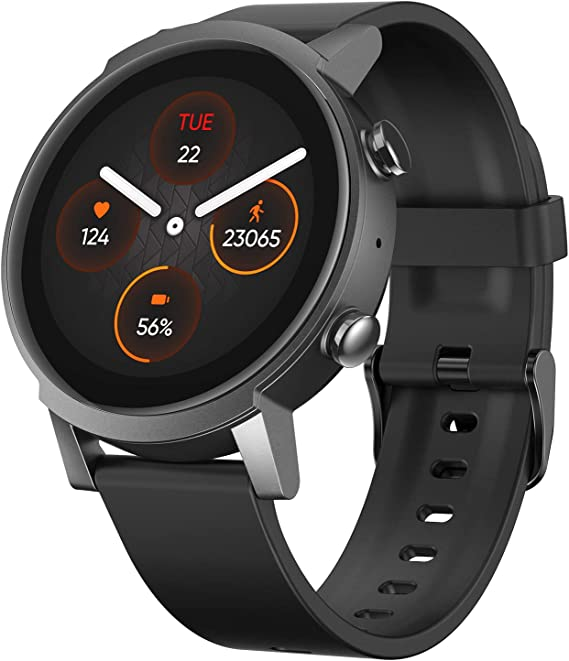
\includegraphics[width=10cm]{images/chapter3/watch.jpg}
    \caption{利用したスマートウォッチ,TicWatchE3}
\end{figure}

\begin{figure}[H]
    \centering
    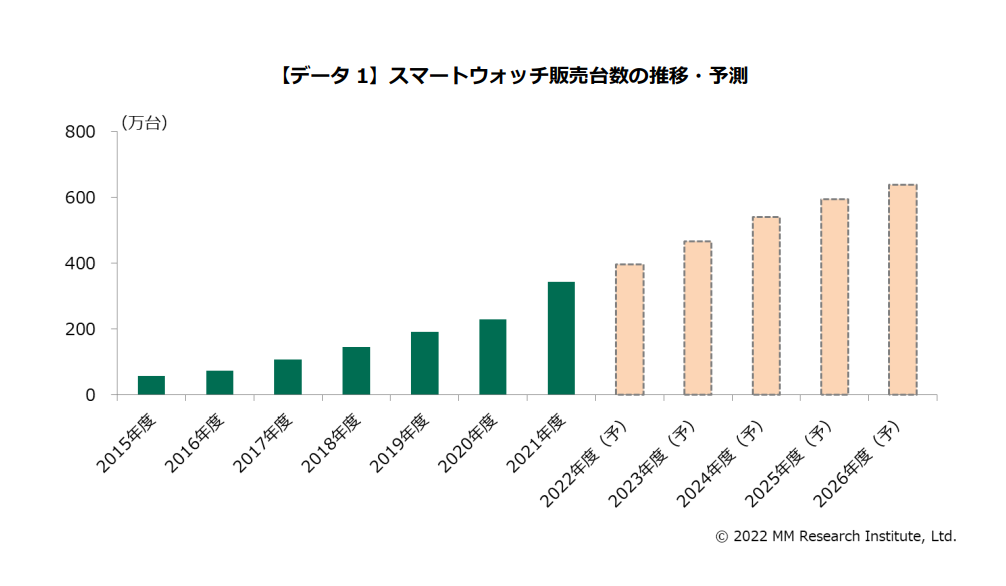
\includegraphics[width=10cm]{images/chapter3/watchreserch.png}
    \caption{スマートウォッチの普及率}
\end{figure}

\section{心拍データについて}

 本節ではシステムを構成する機能のうち,スマートウォッチを使い心拍データを取得する方法,
収集した心拍データから心拍数が上昇している箇所の抽出方法について述べる.

\subsection{心拍データの収集方法}

 スマートウォッチを使い心拍数を計測する方法を述べる.本研究では映画を視聴している時の心拍数を計測するため,
AndroidStudioで心拍数が取得できるアプリを作成した。アプリ画面を図に示す.
センサ取得ボタンを押すことによって腕につけた時の心拍数を心拍という文字の下に表示できる.
csv file nameに保存したいファイル名を記入し記録開始ボタンを押すことで心拍数の記録が始まる.
心拍数を取得中の画面を図に示す.心拍数の計測が終了したらCSV出力のボタンを押し計測を終了する.
取得した心拍データはCSVファイルとなり生体データを管理するサーバへとアップロードされる.

\begin{figure}[H]
    \centering
    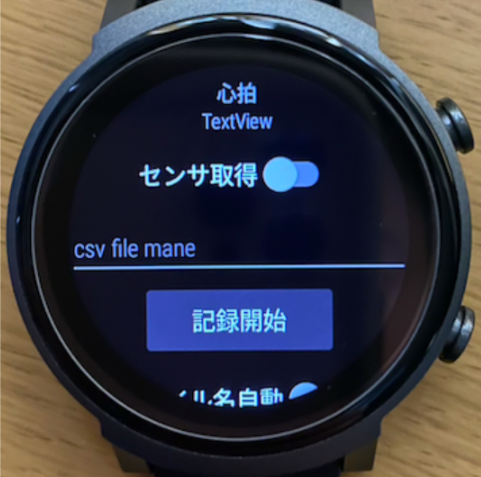
\includegraphics[width=10cm]{images/chapter3/tokei_real.png}
    \caption{心拍数取得画面}
\end{figure}

\begin{figure}[H]
    \centering
    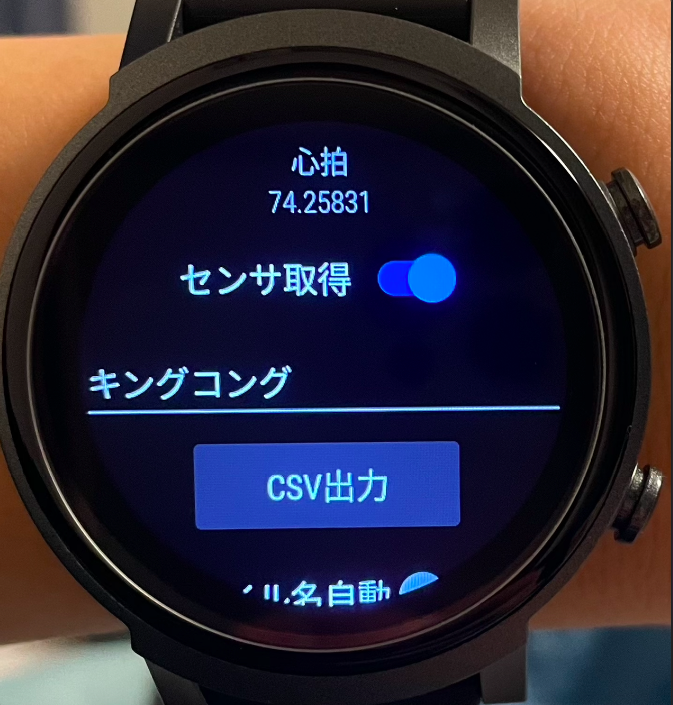
\includegraphics[width=10cm]{images/chapter3/csv.png}
    \caption{心拍数取得中画面}
\end{figure}

\subsection{心拍データの観察}

収集した心拍データを観察する.実際に集めた心拍データの一部をグラフにしたものを表示する図.
映画は「キングコング 髑髏島の巨神」を視聴した人のデータである.集めたデータを観察したところ,人により心拍数の変動が様々であった.
図のように盛り上がりを見せるシーンのみ心拍数が上昇しそれ以外は比較的落ち着いている人がいたが,
図のように常に心拍数が上昇と下降を繰り返しており盛り上がっている箇所が把握できない人や、図のように盛り上がりを見せるシーンでは心拍数が大幅に上昇し、
それ以外は上昇と下降を繰り返している人もいた.また人によって映画視聴中の平均心拍数にばらつきがあった.
映画の盛り上がるシーンと心拍数の関係を比較したところ,盛り上がりを見せるシーンで心拍数が上昇している人がいた.
図と図は数分の差はあったものの盛り上がるシーンで平均の心拍数よりも上昇していた.
これより人によって差はあるが映画を視聴している時の盛り上がるシーンでは心拍数が上昇することがわかった.

\begin{figure}[H]
    \centering
    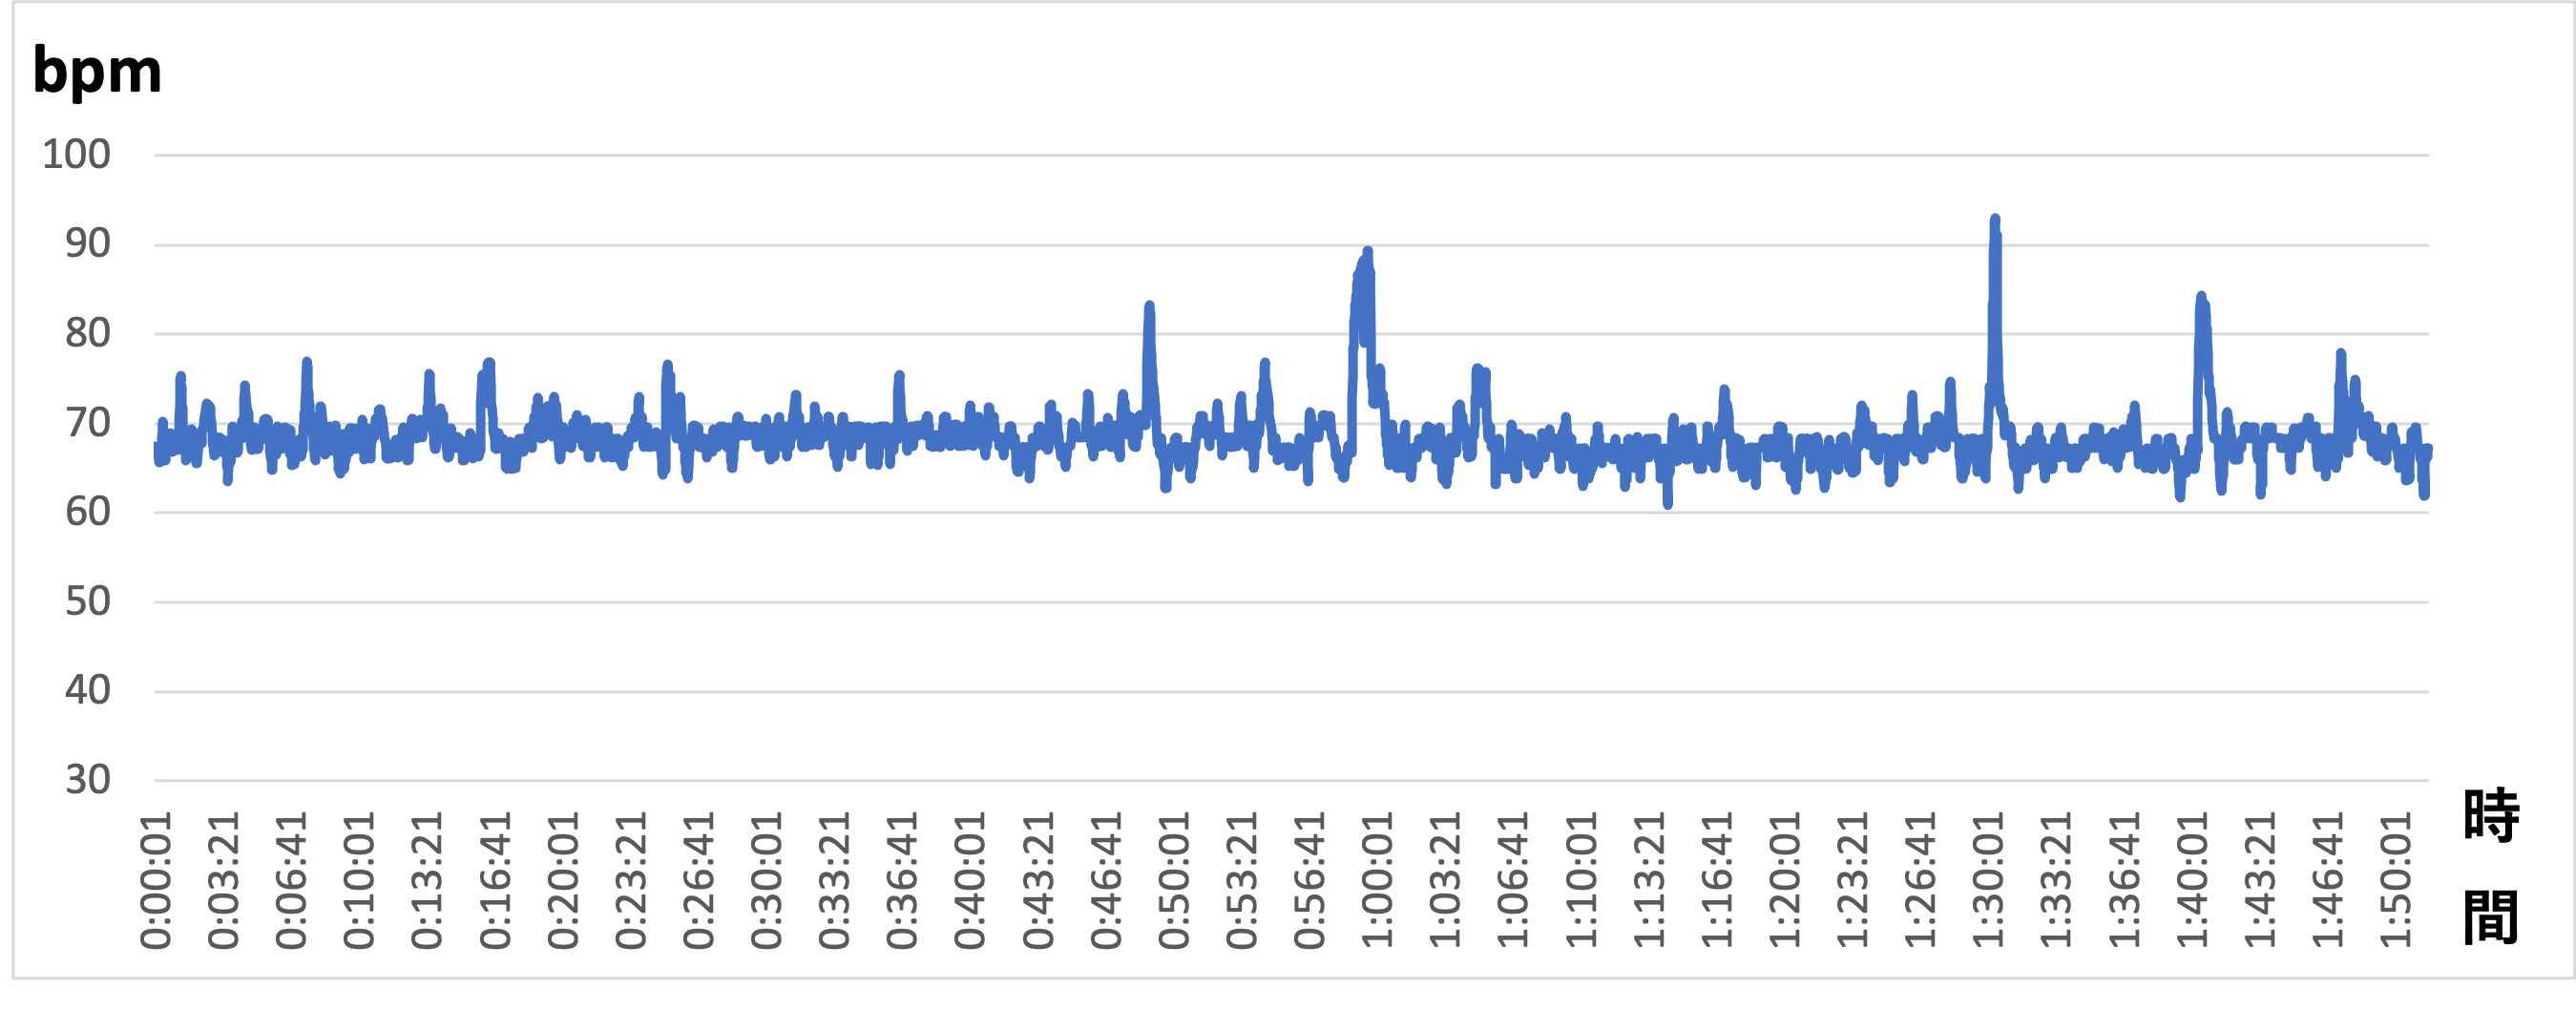
\includegraphics[width=10cm]{images/chapter3/gurafu2.png}
    \caption{キングコングを視聴した時の1人目心拍数のグラフ}
\end{figure}

\begin{figure}[H]
    \centering
    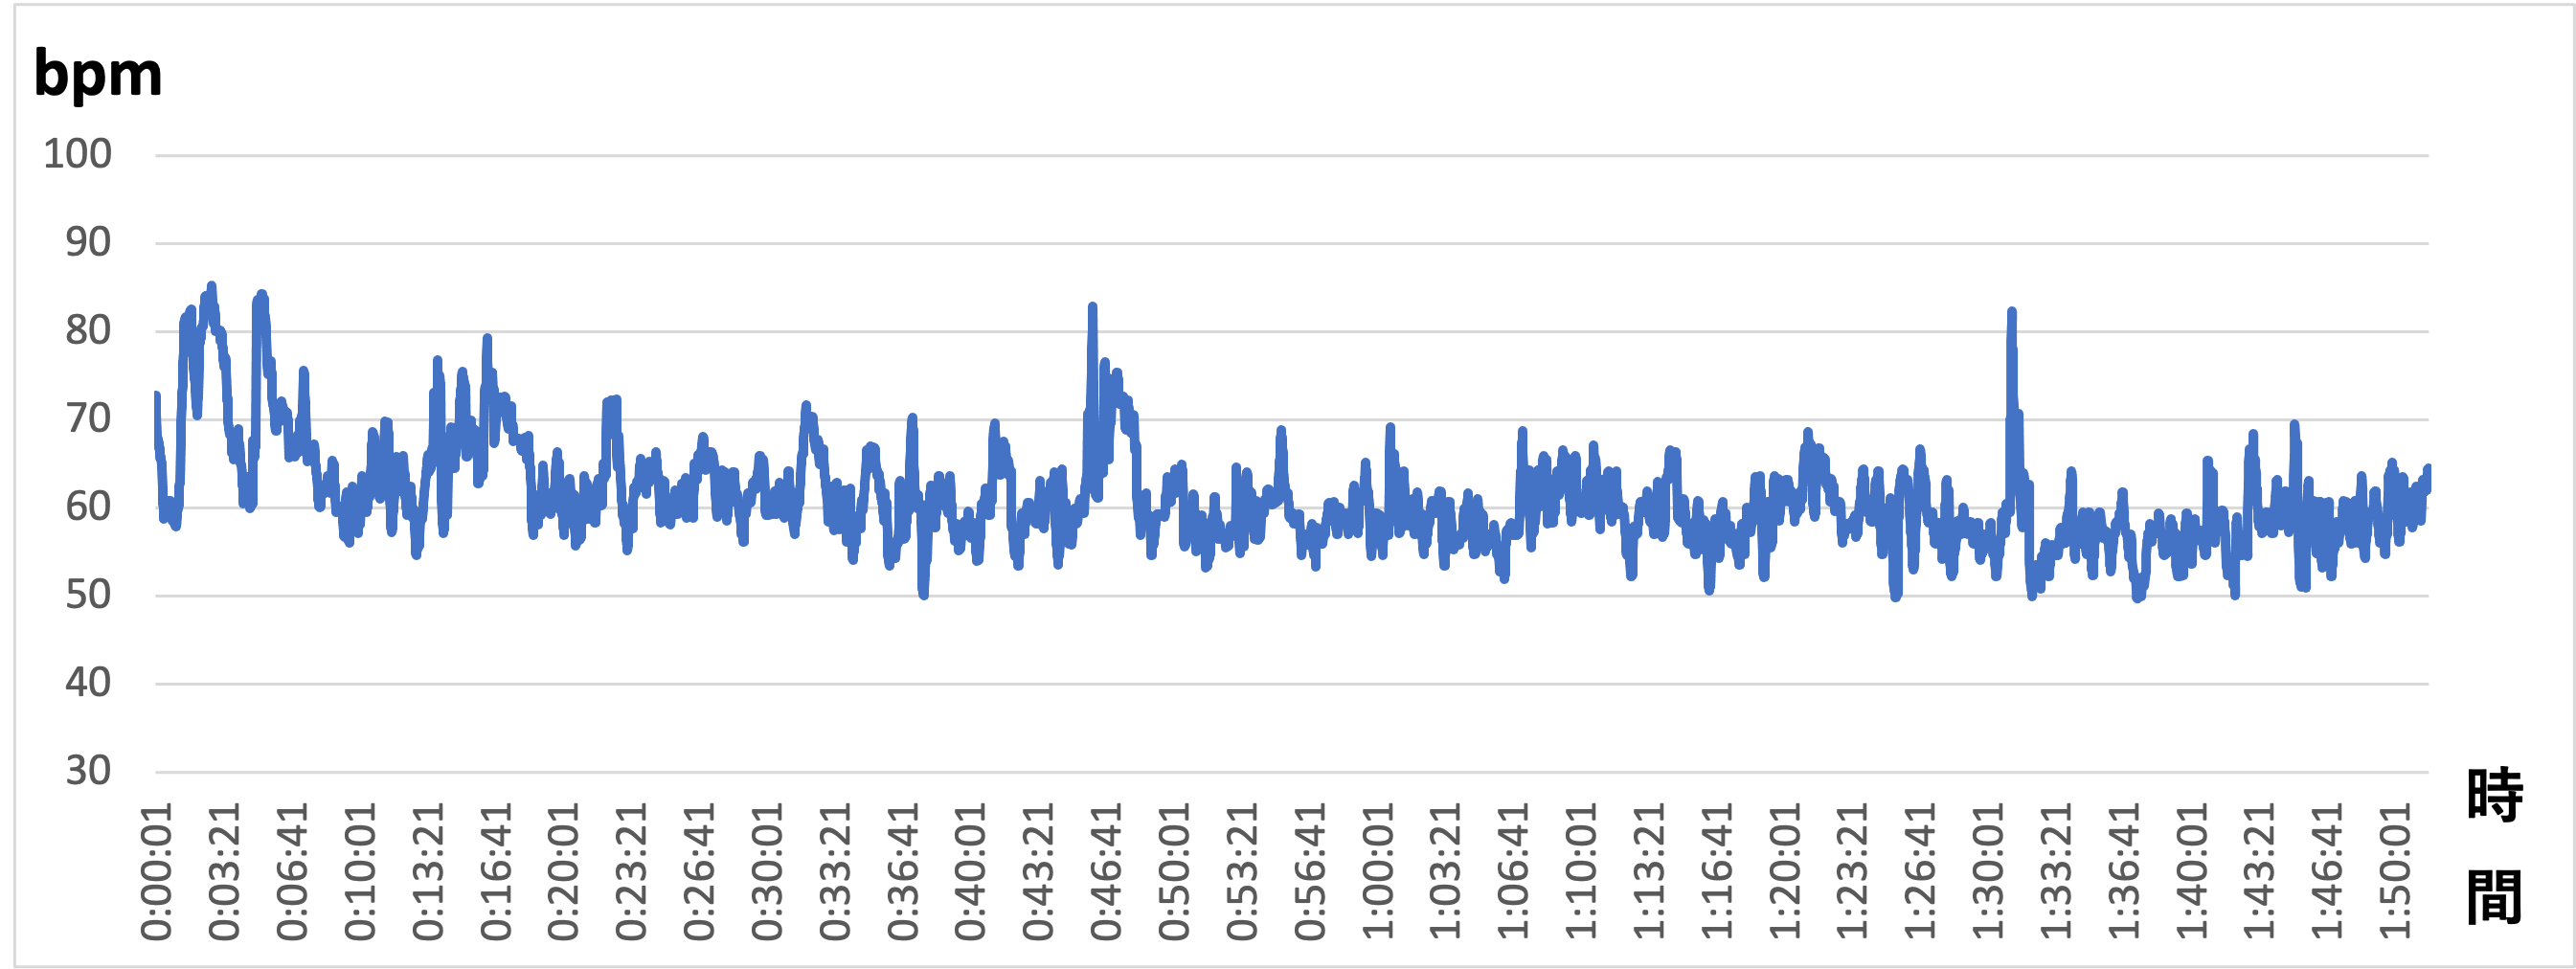
\includegraphics[width=10cm]{images/chapter3/gurafu.png}
    \caption{キングコングを視聴した時の2人目心拍数のグラフ}
\end{figure}

\begin{figure}[H]
    \centering
    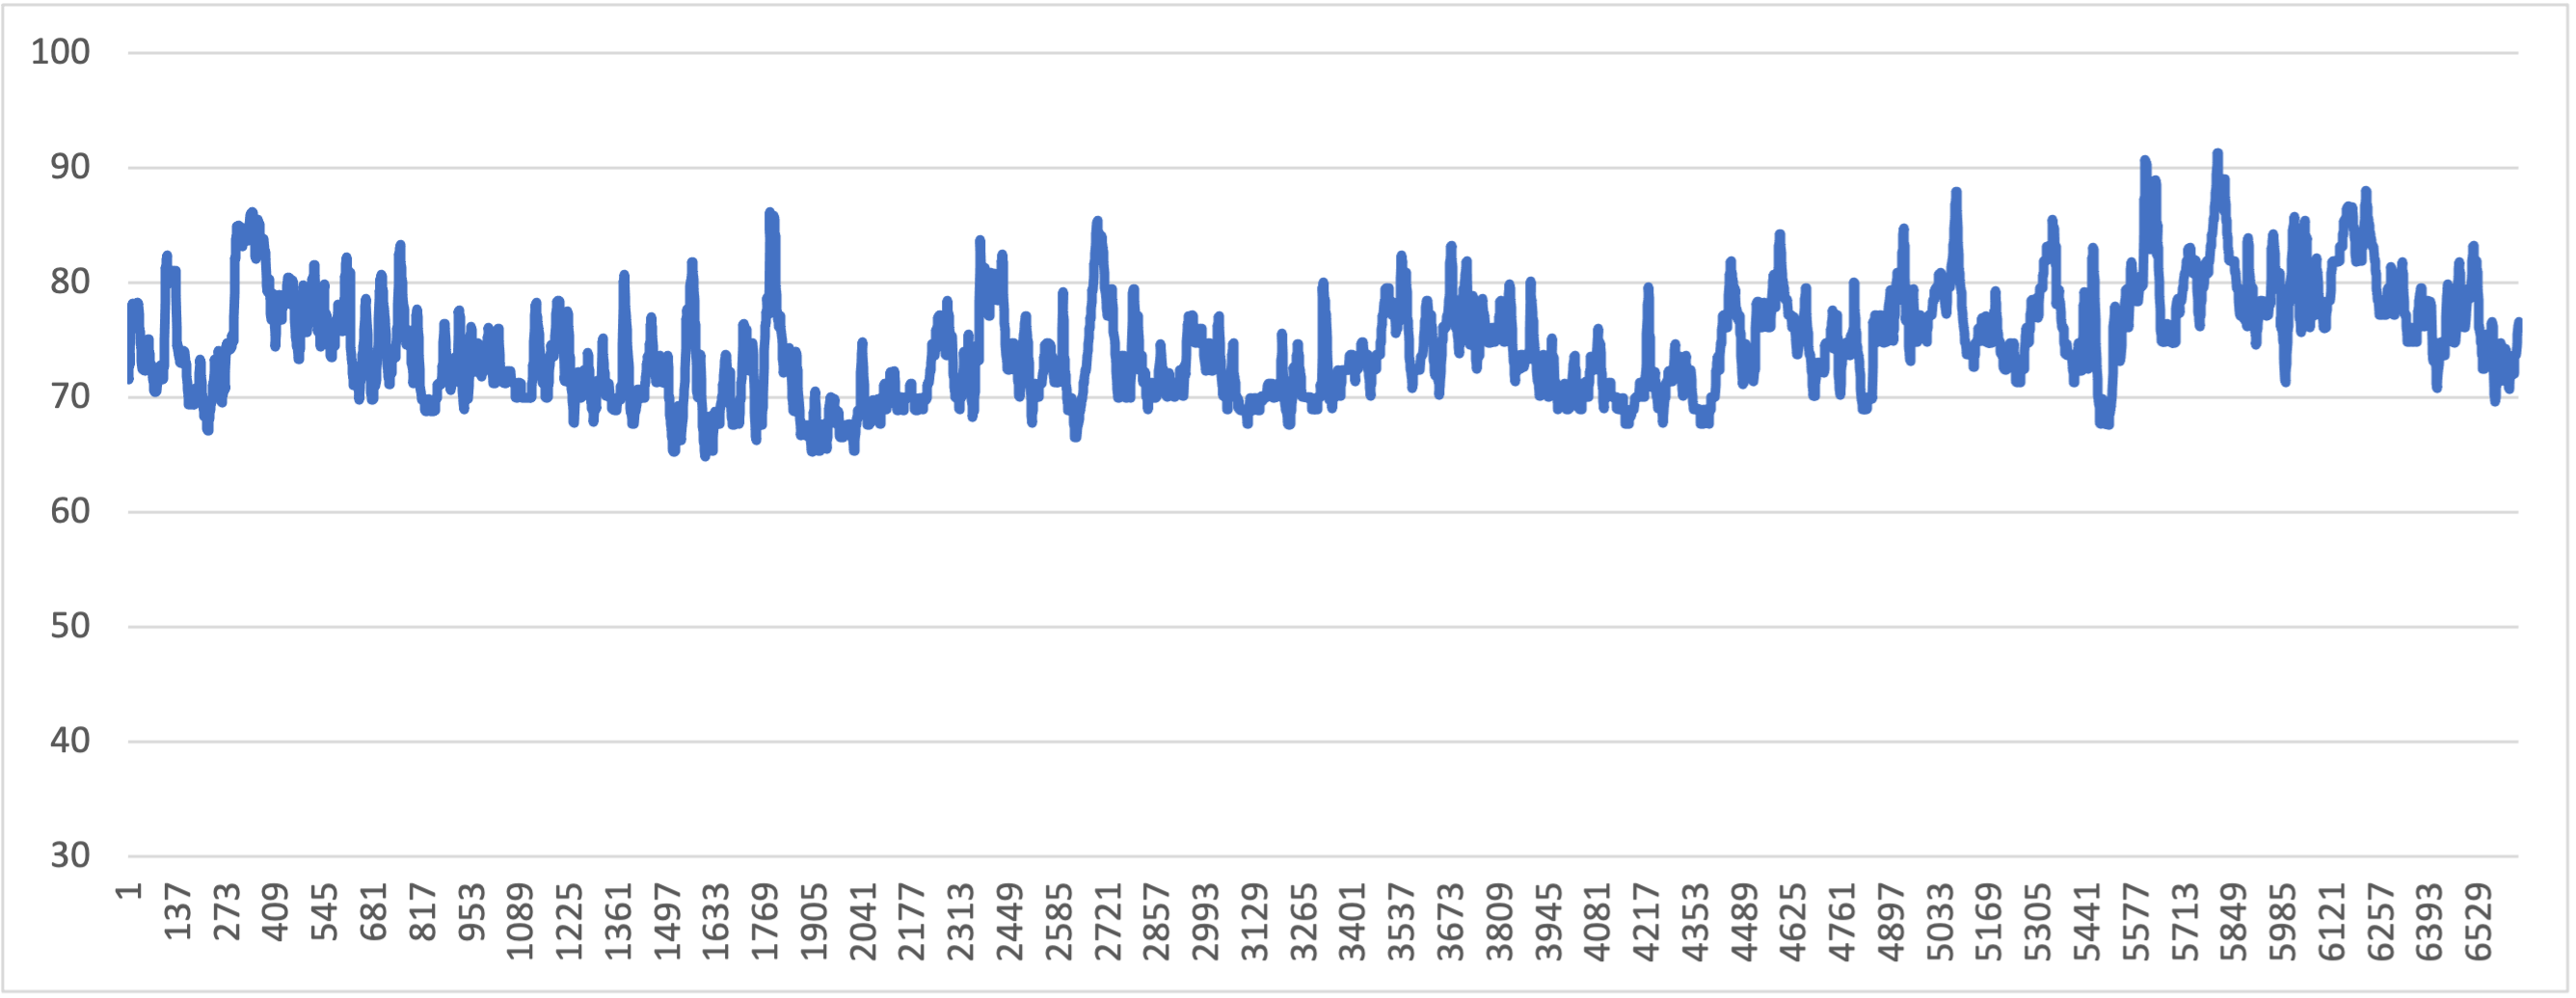
\includegraphics[width=10cm]{images/chapter3/gurafu1.png}
    \caption{キングコングを視聴した時の3人目心拍数のグラフ}
\end{figure}

\subsection{心拍数上昇箇所の抽出処理}
 収集した心拍データを基に,エフェクト表示に適した形式にするため心拍数が上昇している箇所を抽出するための処理を行う.
収集した心拍数の CSV データをエフェクト表示に適したJSON データにする.
エフェクト表示用に作成したデスクトップアプリの都合上本研究ではJSONデータに変換する.
まず,サーバから心拍数のCSVデータを取得し心拍数が上昇している箇所の抽出を行う.心拍数上昇箇所の抽出処理の方法を図 に示す.
収集した心拍データを観察し,心拍数が上昇している箇所の抜き出し方法を決定した.人により平均の心拍数はさまざまであったため,
心拍数が上昇している箇所を見つけ出すようまず安静時の心拍数を取得する.安静時の心拍数は,映画を視聴する前の1分間動かない状態で心拍数を計測し取得する.
その安静時の平均心拍数からどれだけ心拍数が上昇したかを抽出する.これにより心拍数が高い人も低い人も同じ抽出処理が可能になる.
表に今回作成したモデルの定義を示す.from toの形式で心拍数が閾値を超えていた時間を示す.
時間は映画が始まってからの経過時間でエフェクト表示するため相対時間にした.今回from toの形式にしたのは,
エフェクトを映画画面に重畳する際にエフェクト表示する時間を心拍数が閾値を超えていた時間の範囲で表示できるようにするためである.
effectlevelで表示するエフェクトを決定する.effectlevelは表のように心拍数を閾値と比較する.閾値は収集した心拍データを基に設定した.
心拍数の上昇具合で表示するエフェクトを変更するため,1から3までのレベル分けをした.
本研究ではエフェクトを3段階にし心拍数のレベルに応じて表示するエフェクトが変更される.安静時の平均心拍数よりも心拍数が16bpm以上高い時をレベル3,
14bmp以上をレベル2,12bpm 以上をレベル1とする.実際に心拍数上昇箇所の抽出処理をした後のデータを図に示す.


\begin{figure}[H]
    \centering
    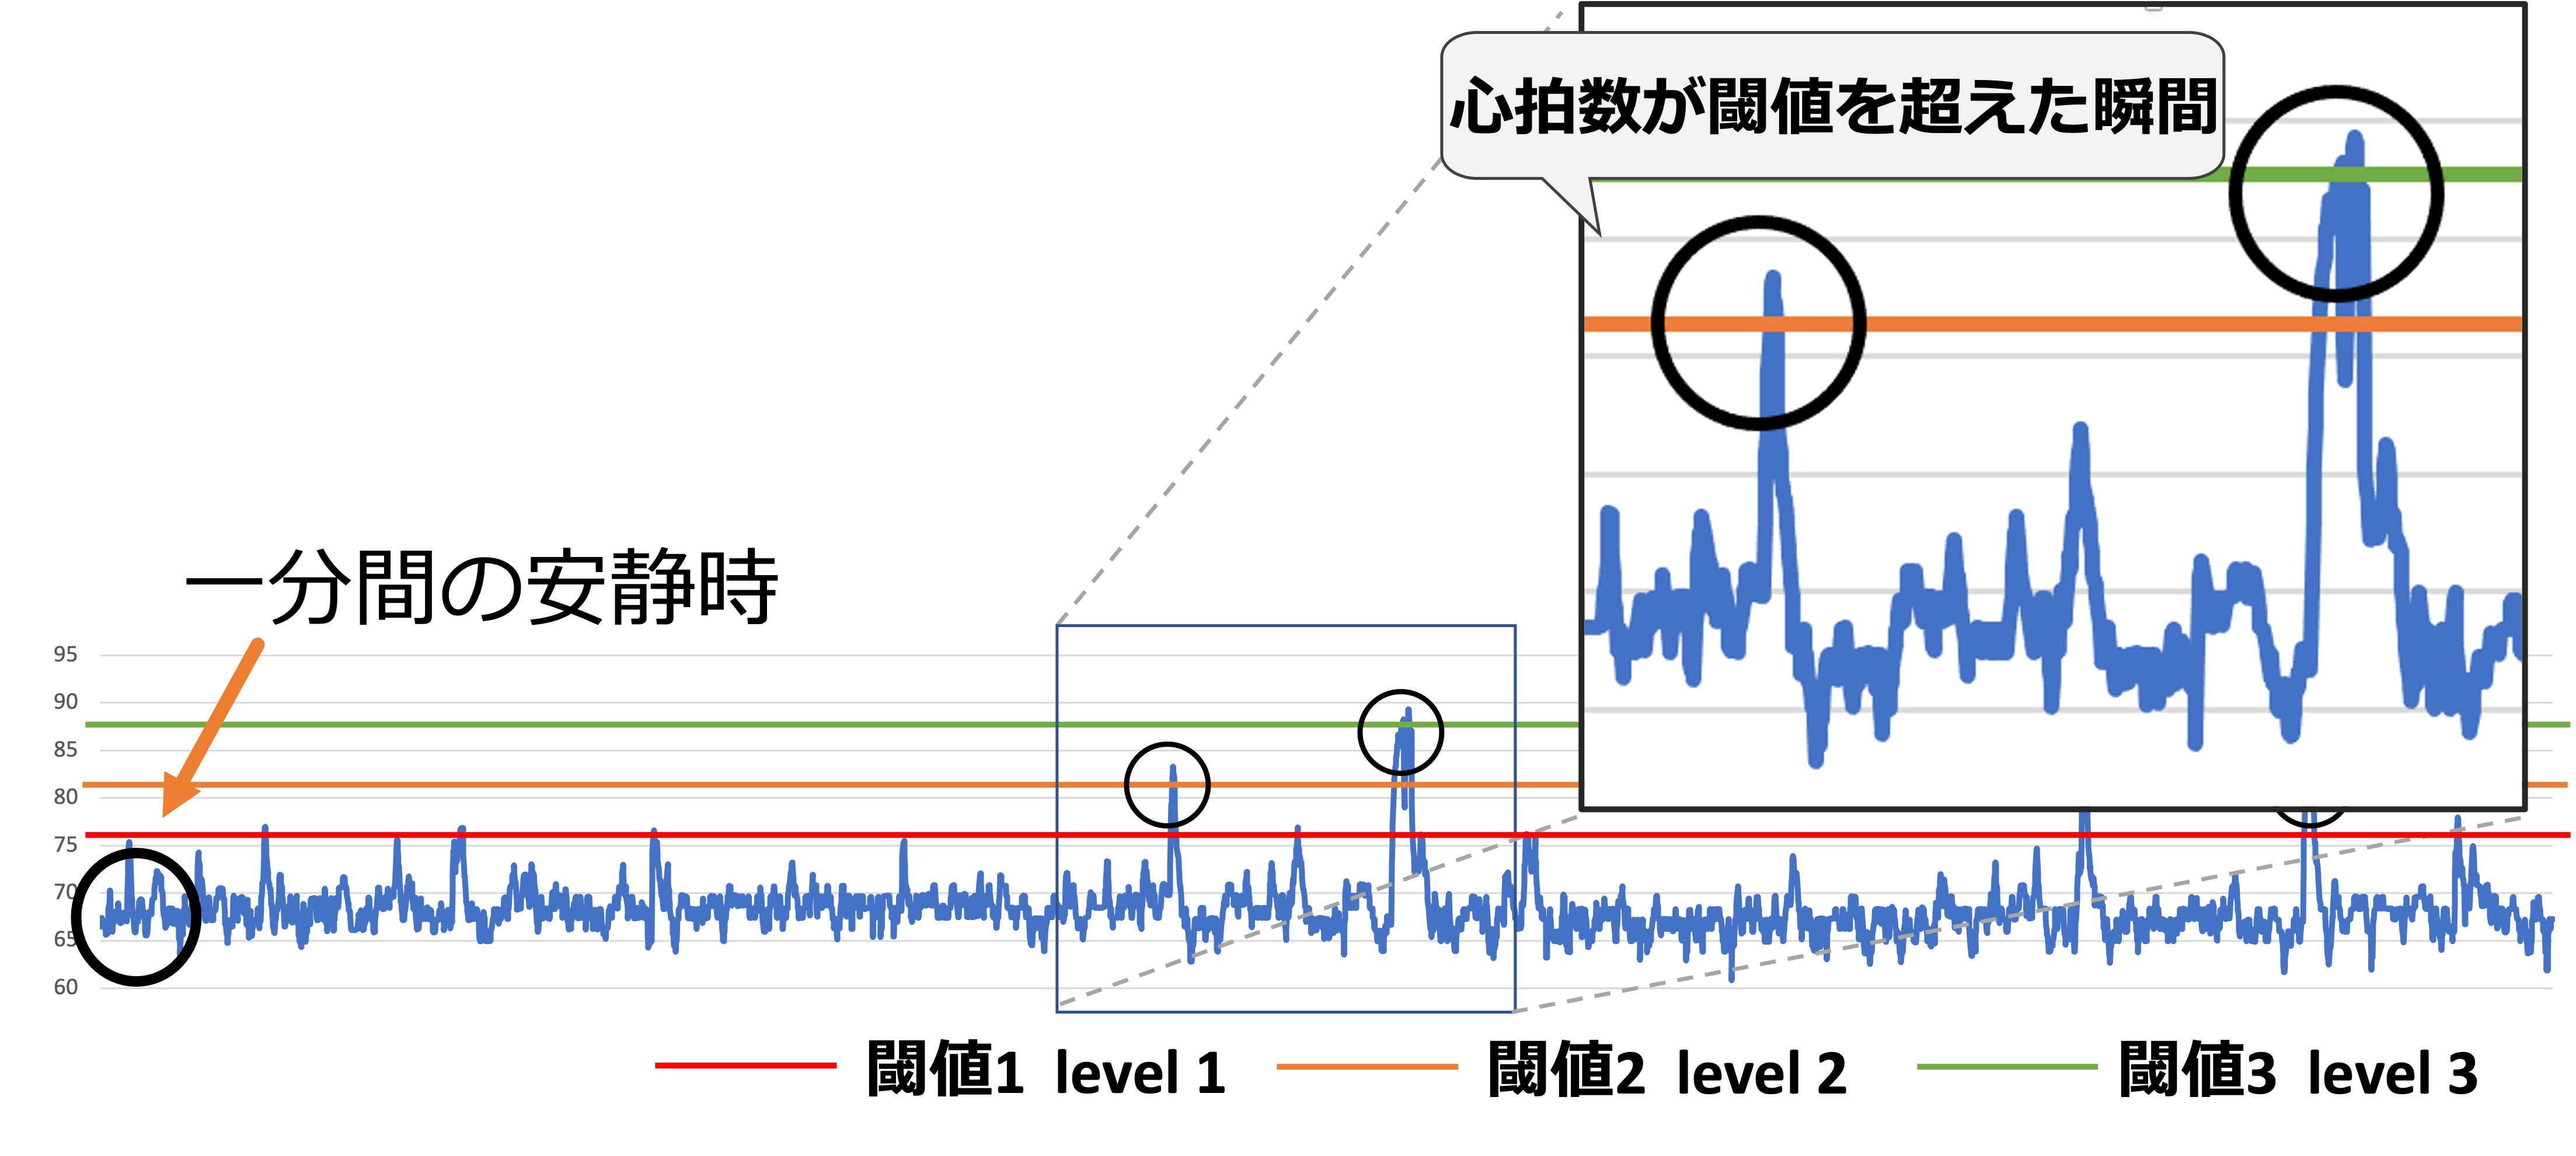
\includegraphics[width=10cm]{images/chapter3/haisyutusyori.png}
    \caption{心拍数上昇箇所の抽出処理}
\end{figure}

\begin{figure}[H]
    \centering
    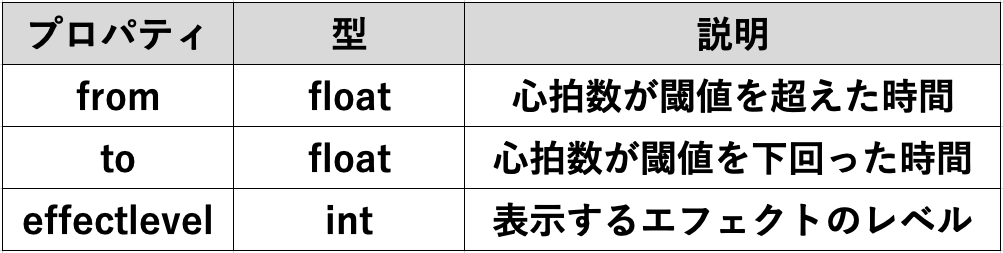
\includegraphics[width=10cm]{images/chapter3/propaty.png}
    \caption{心拍データのモデルの型定義}
\end{figure}

\begin{figure}[H]
    \centering
    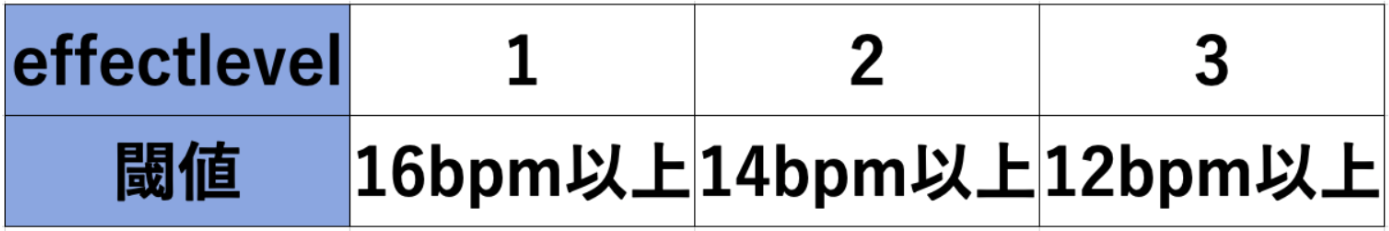
\includegraphics[width=10cm]{images/chapter3/effectlevel.png}
    \caption{閾値の判別}
\end{figure}


\begin{figure}[H]
    \centering
    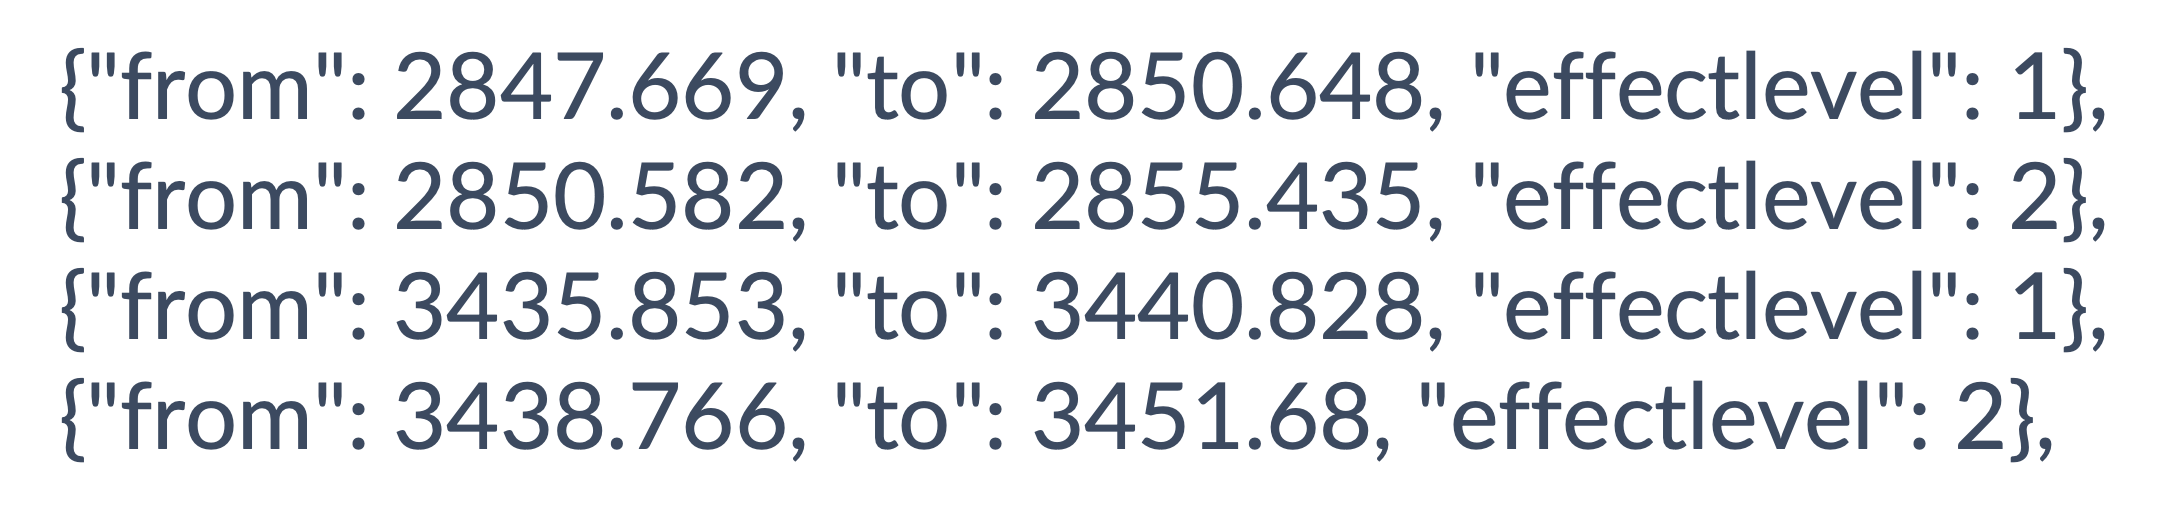
\includegraphics[width=10cm]{images/chapter3/level.png}
    \caption{心拍数上昇箇所の抽出処理をした結果}
\end{figure}


 エフェクト表示に適した形式にするため、心拍数上昇箇所の抽出処理したJSONデータを一つのJSONデータにまとめる.
これにより一つのコンテンツに一個のJSONデータが作られる.このデータを使いエフェクトを映画画面に重畳する.

\begin{figure}[H]
    \centering
    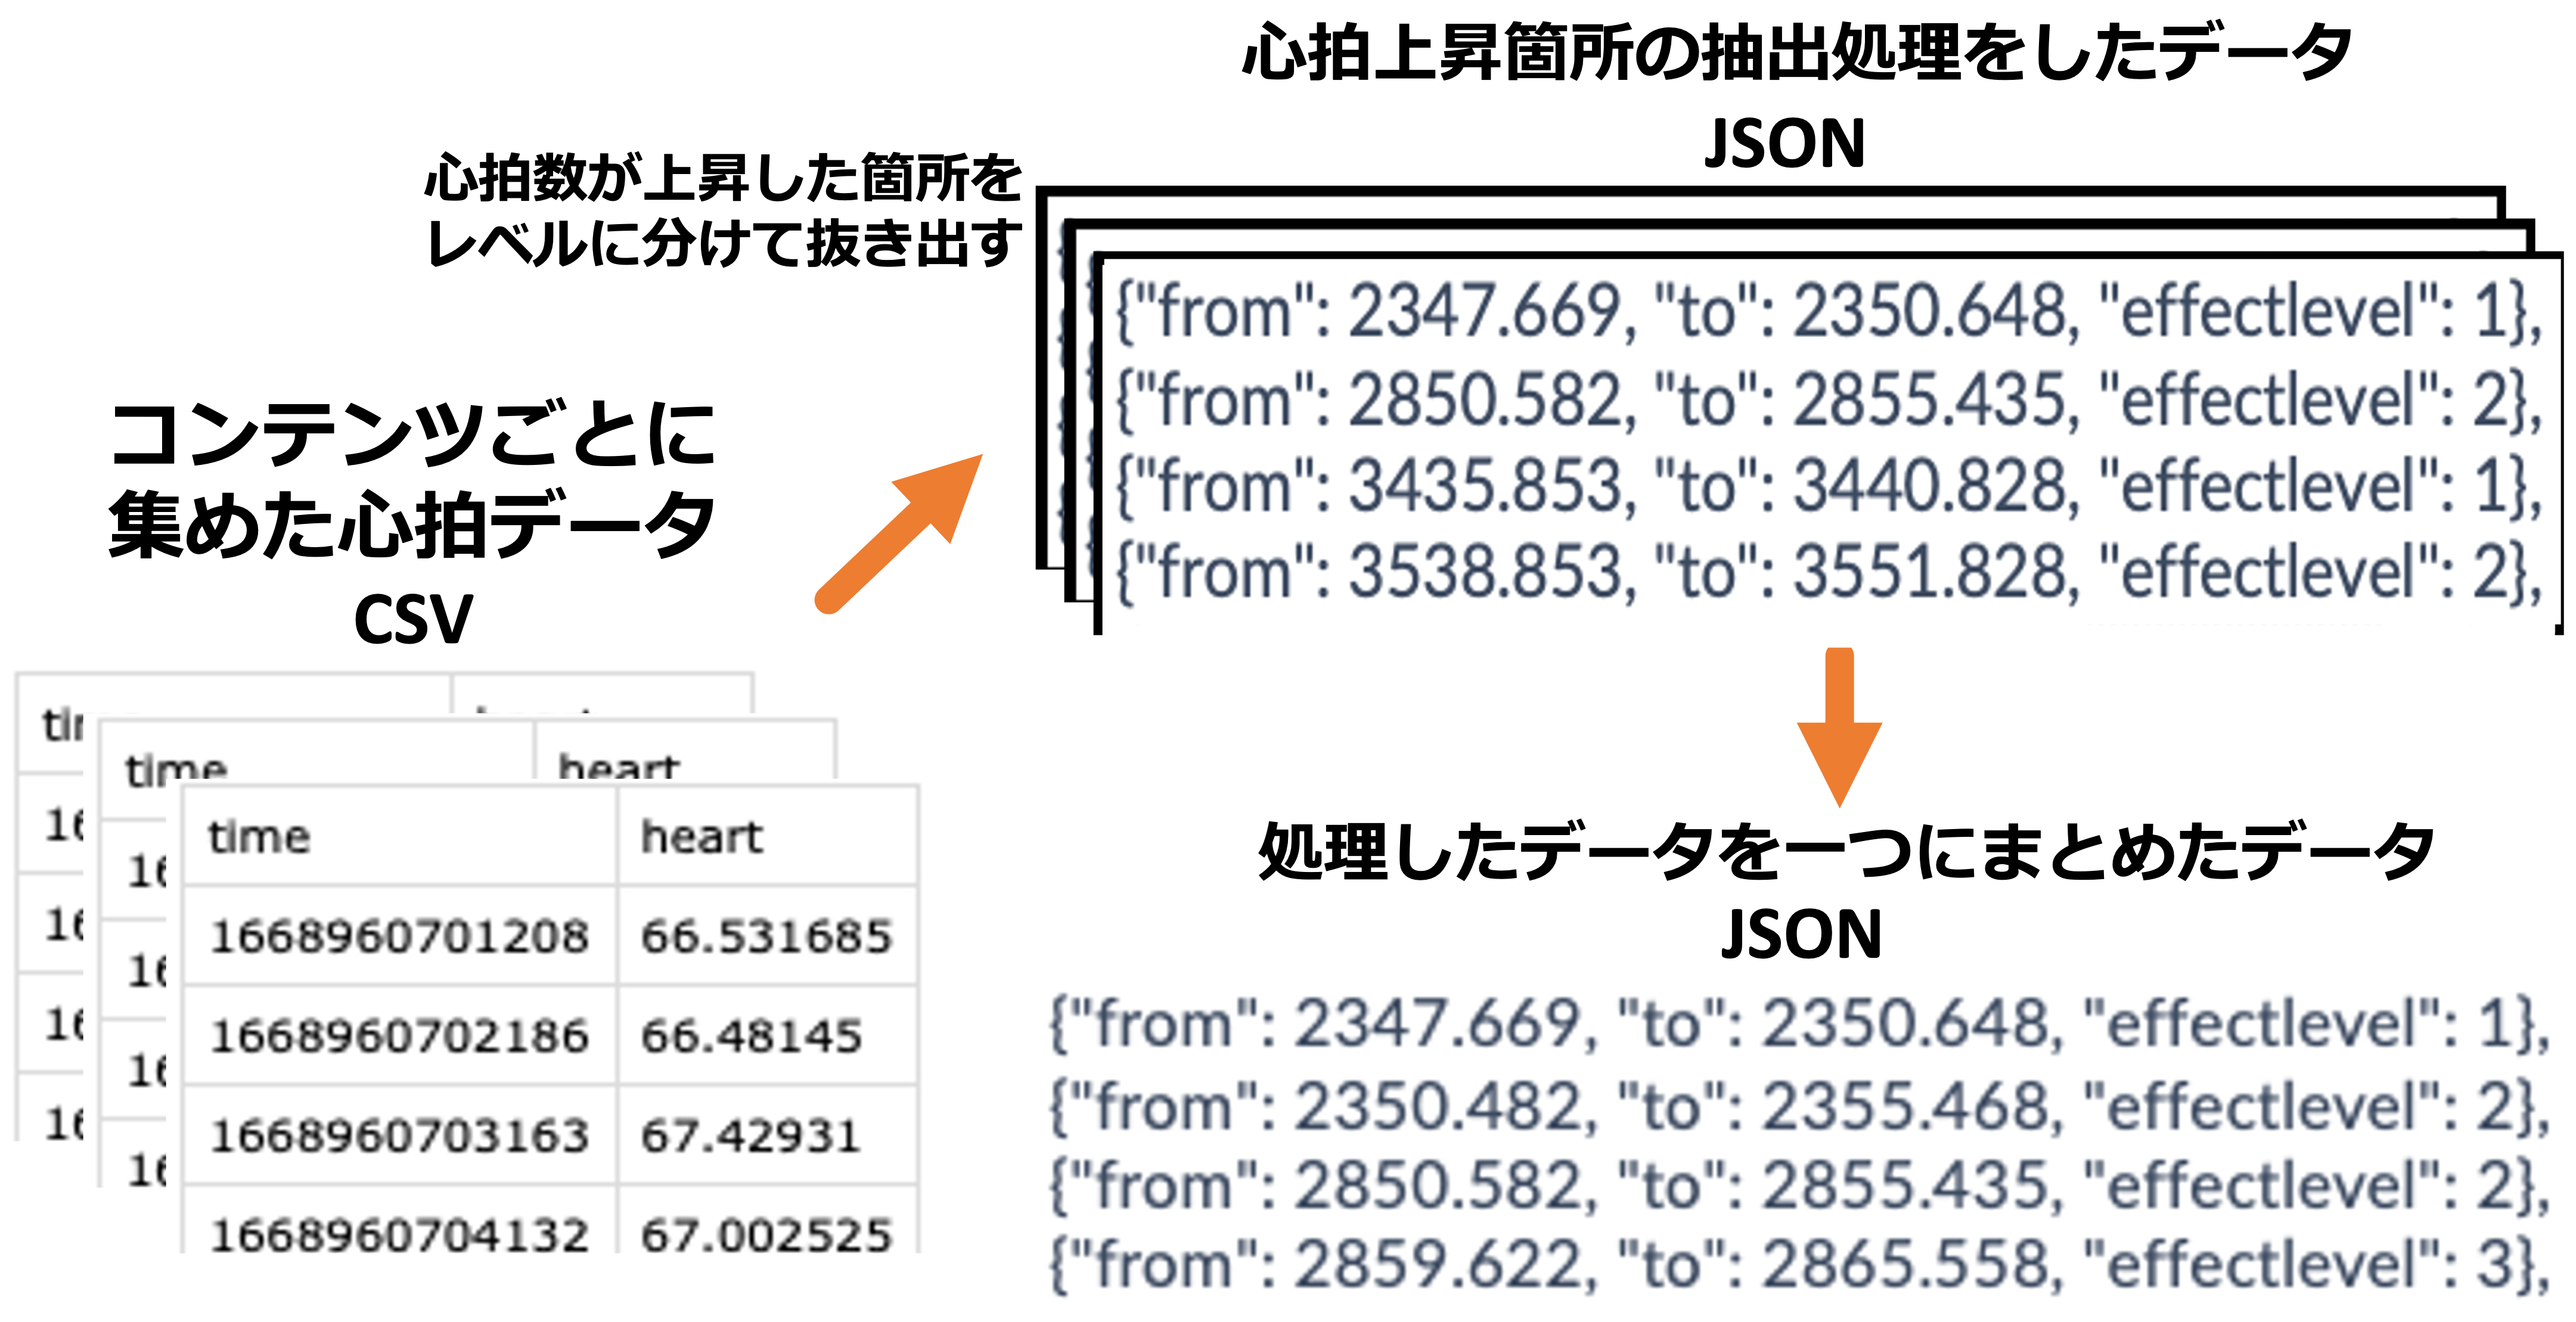
\includegraphics[width=10cm]{images/chapter3/system.png}
    \caption{心拍データの概要図}
\end{figure}







\section{エフェクト表示}
\subsection{本研究のシステム構成}
エフェクト表示方法として,カテゴリやレベルごとにエフェクトを用意し,動画として重畳表示しているが,レベル分けを行ったためエフェクトをダイナミックに生成できず,細かな心拍数変化を表示できていない.
本研究では,視聴者ごとにエフェクトを自由に選択できるようにするためElectronを使用し,PCを使用する環境下での重畳表示が可能になっている.
Electronを起動し,視聴する動画コンテンツを選択し,視聴する映画のジャンルに合わせるエフェクトを選択し,Playをクリックし,エフェクト重畳が開始するようになっている.実際の動作画面を図に示す.

\begin{figure}[H]
    \centering
    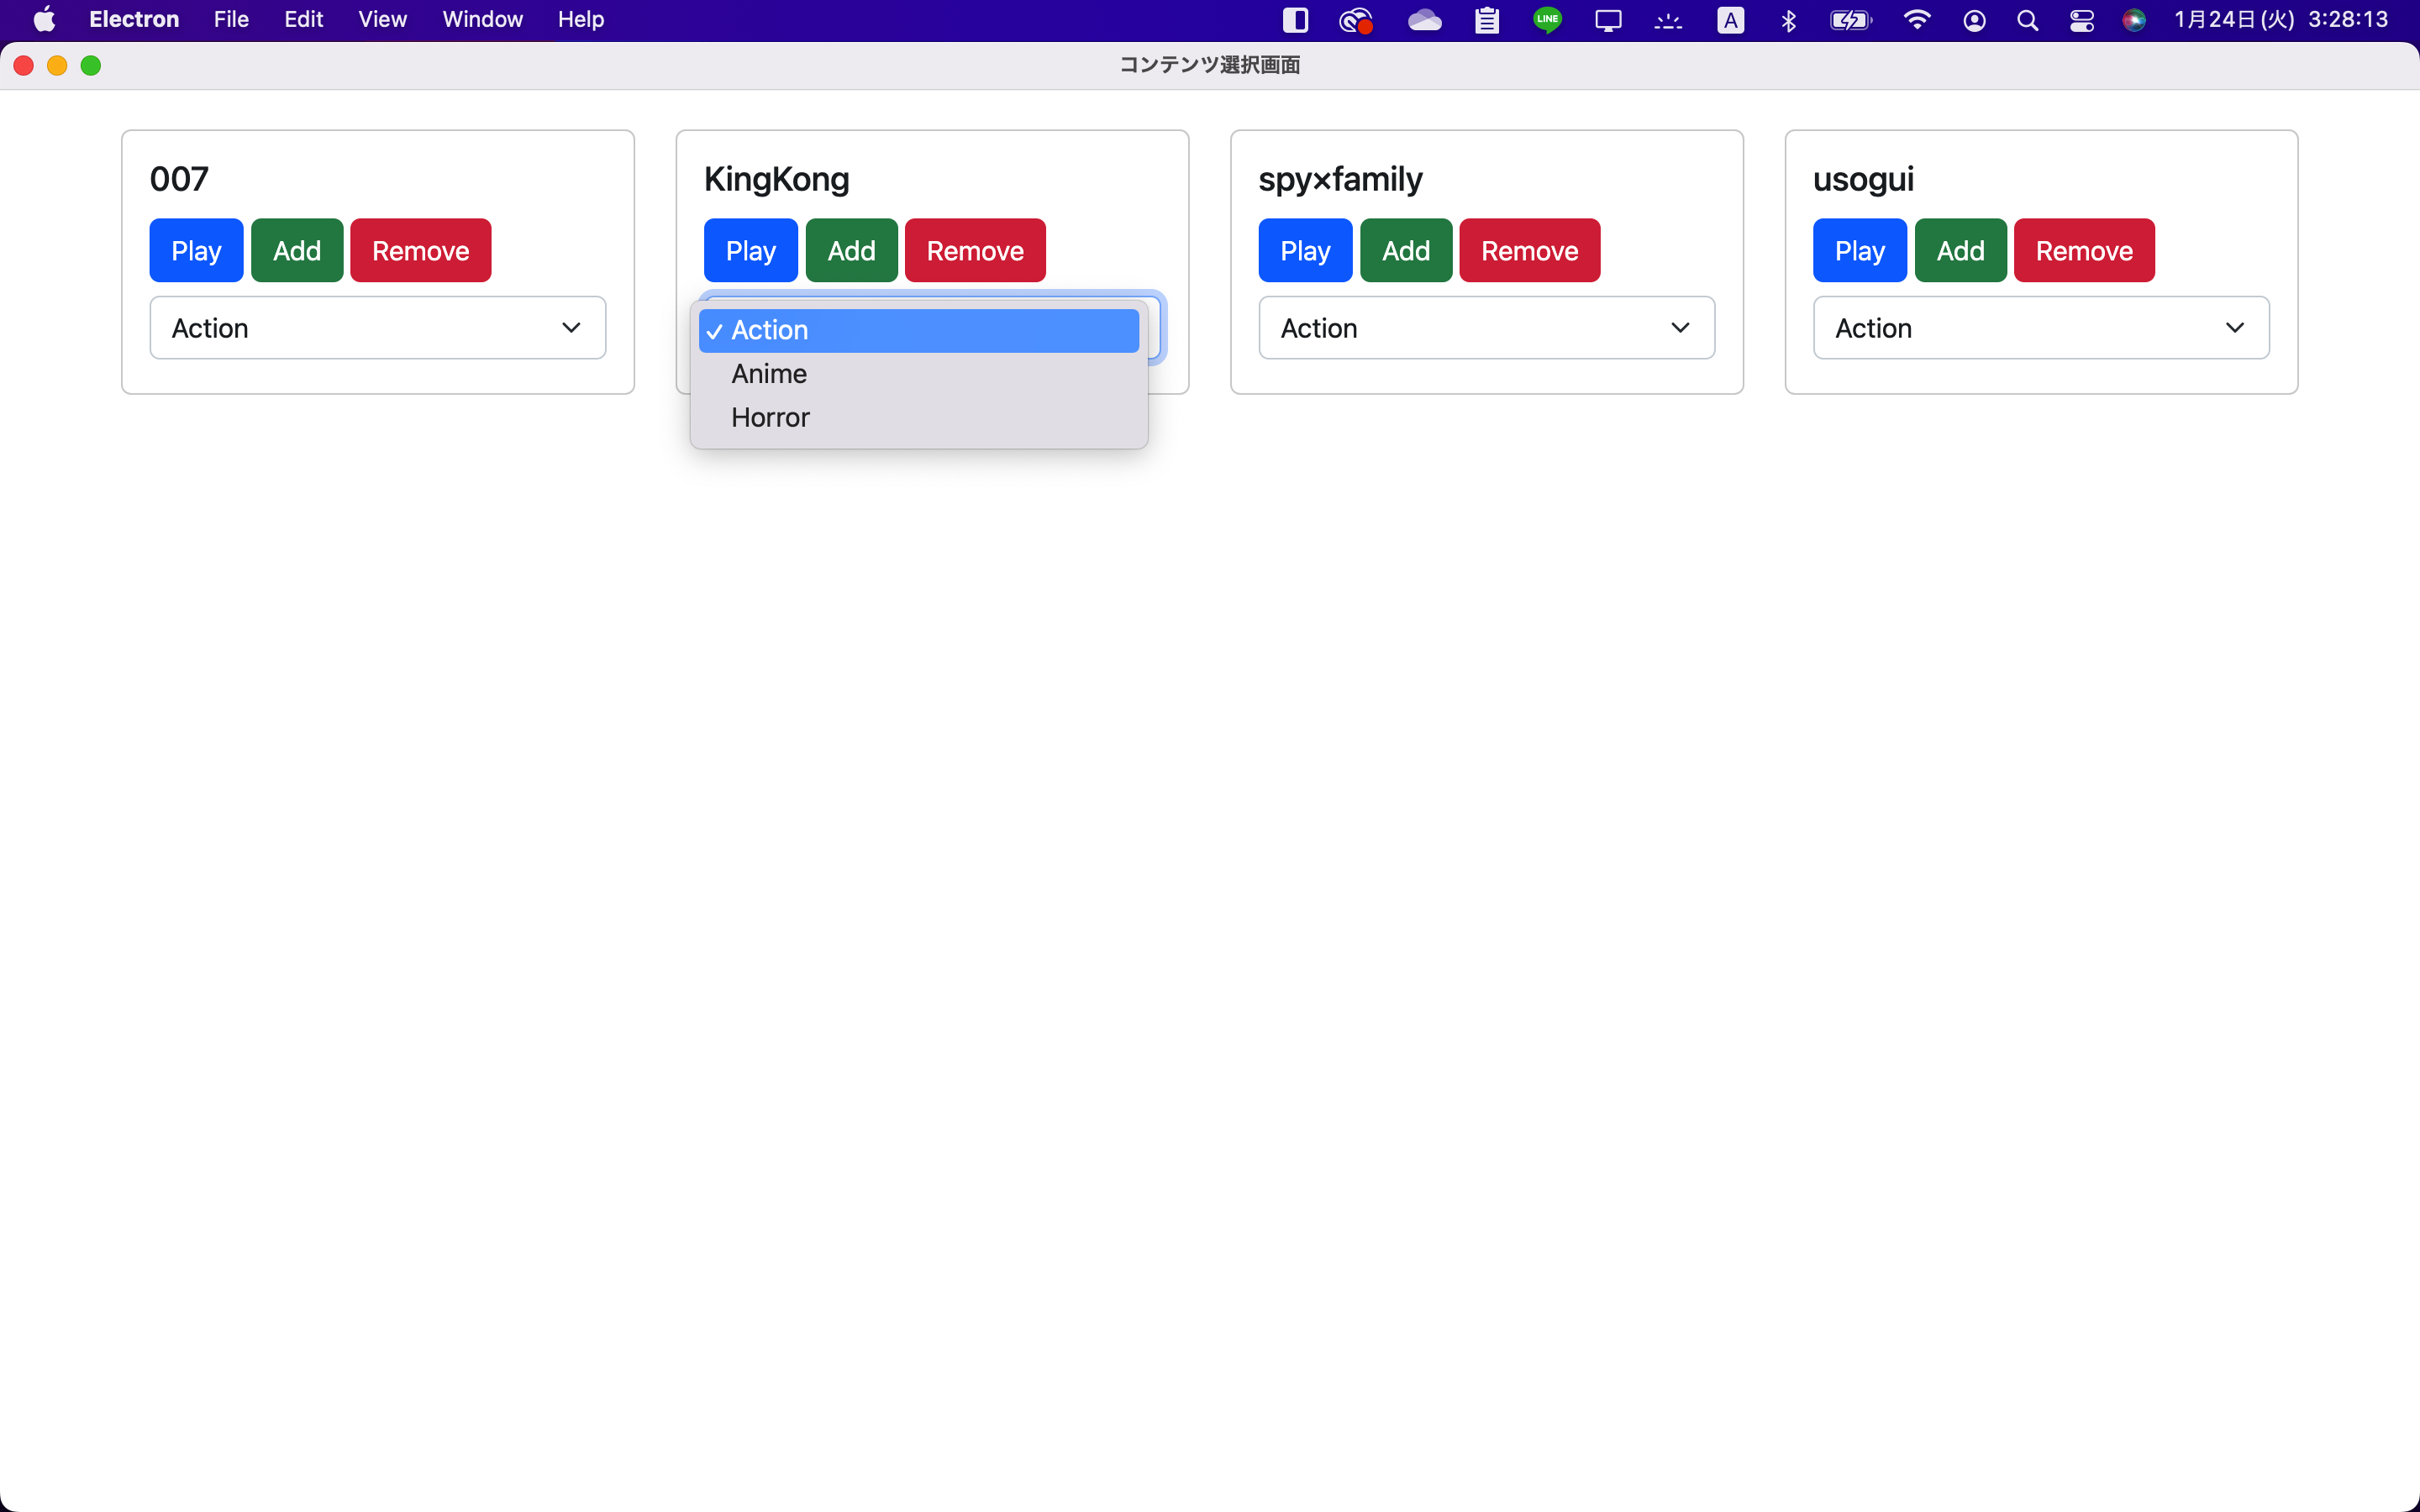
\includegraphics[width=10cm]{images/chapter3/contents.jpg}
    \caption{コンテンツ選択画面}
\end{figure}

\subsection{エフェクト種類}
エフェクトの種類としてAction, Anime, Horrorの3種類に分け見る映画のジャンルを選択可能にした.選択できるようにした理由として,視聴ジャンルによって同じエフェクト効果を表示した際に,エフェクトが映像視聴の際に邪魔になってしまう点が挙げられる.
エフェクトの目的として,Actionのエフェクトは迫力・緊迫感を与え,Animeのエフェクトは面白さを与える,Horrorのエフェクトは恐怖を軽減させる目的として制作した.心拍データの処理の際に1から3までのレベル分けの結果でエフェクトが変更される.1から3に分けた際に1の結果が出力された時間はエフェクトを透過し映像視聴の邪魔にならないように制作し,2と3の結果が出力されている時のみに2段階に分けエフェクトが表示されるように制作した.
実際の画面にエフェクトを表示した例を図に示す,Actionのエフェクトは赤色の不透明度を上げ,色相彩度を上げる.Animeのエフェクトは効果線を増やす.Horrorのエフェクトは不透明度を下げ,ぼかしの不透明度を上げるように制作した.Action, Horrorのエフェクト制作ではAfter Effectsを使用しフラクタルノイズ効果,色被り補正で制作.Animeのエフェクト制作ではIllustratorを使用し効果線を制作した.

\begin{figure}[H]
    \centering
    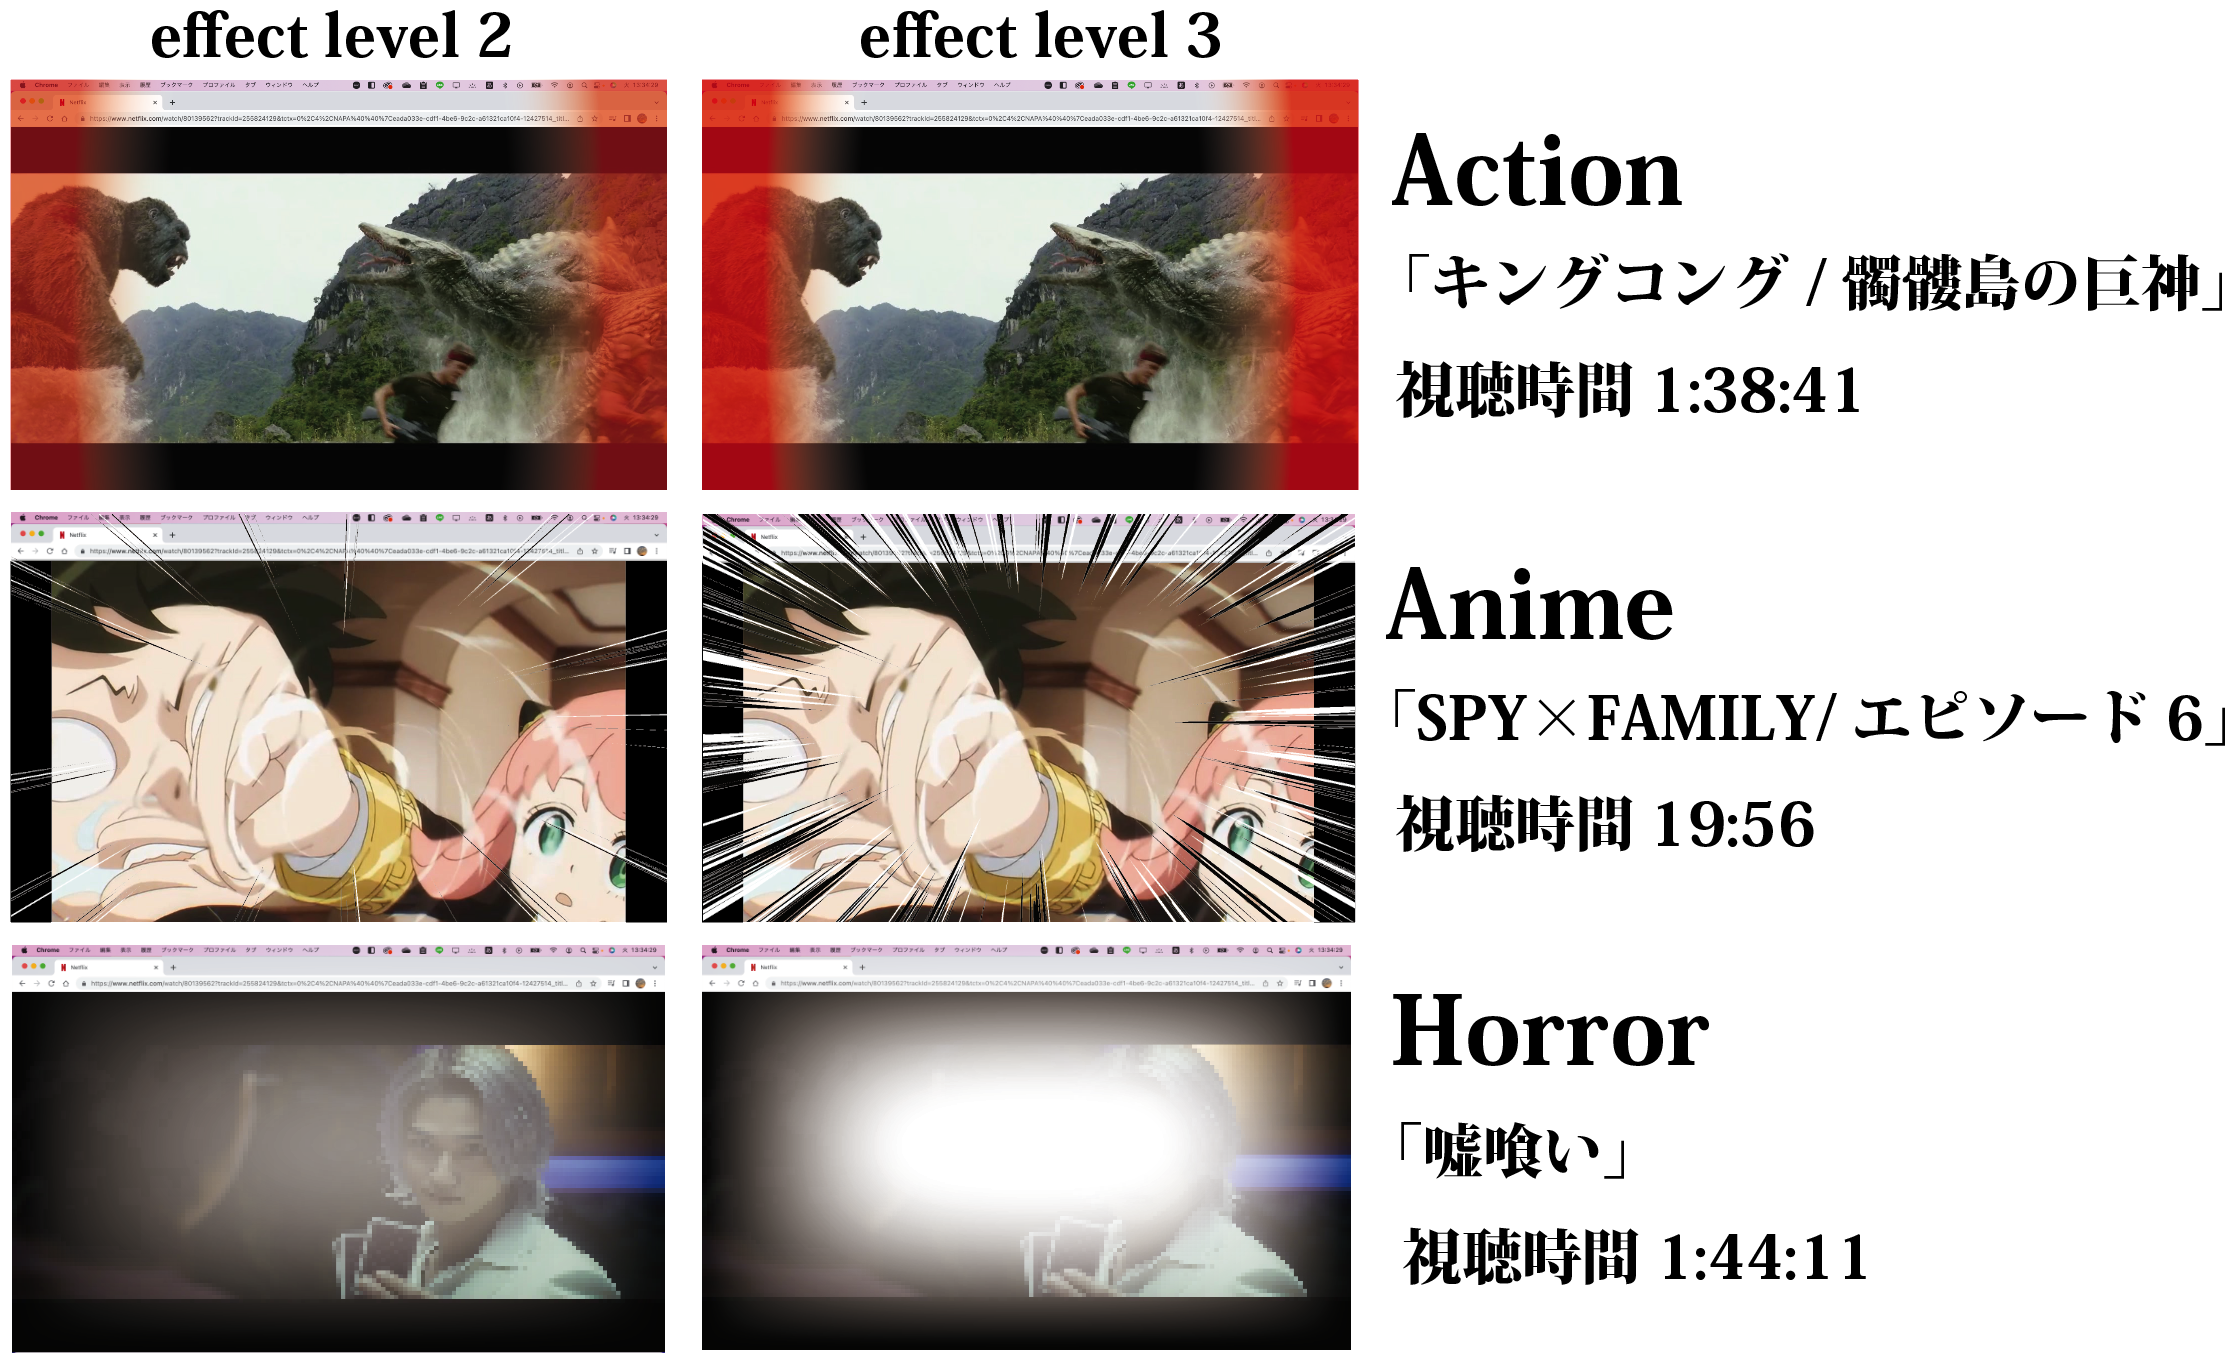
\includegraphics[width=10cm]{images/chapter3/effectjissou.jpg}
    \caption{実装画面}
\end{figure}